% Source-faithful schematic draft, not to scale.
% source_id=src-bfaf1f0ca2f3b8edd4a2455d39b464722513d2bb05efe36769938f1f187729e5
% source_sha256=fca2f5abda4a5e4982176417bf2f33b6b248847bffb0dcd09ae089c4f6a85b6e; PDF p.2; Q20.
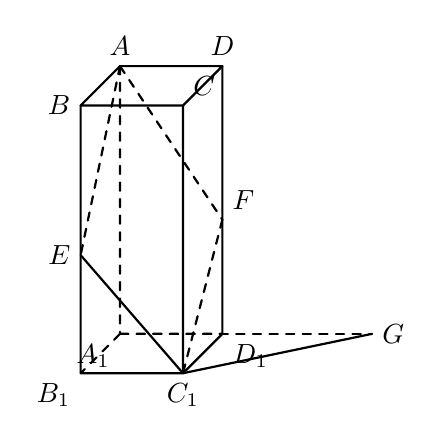
\begin{tikzpicture}[line cap=round,line join=round,thick]
  \coordinate (A) at (0,3.2); \coordinate (B) at (-0.5,2.7);
  \coordinate (C) at (0.8,2.7); \coordinate (D) at (1.3,3.2);
  \coordinate (A1) at (0,-0.2); \coordinate (B1) at (-0.5,-0.7);
  \coordinate (C1) at (0.8,-0.7); \coordinate (D1) at (1.3,-0.2);
  \coordinate (E) at (-0.5,0.8); \coordinate (F) at (1.3,1.25);
  \coordinate (G) at (3.2,-0.2);
  % Prism faces and edges. Rear/hidden edges are dashed as in the source.
  \draw (A)--(B)--(C)--(D)--cycle;
  \draw (B)--(B1) (C)--(C1) (D)--(D1) (B1)--(C1)--(D1);
  \draw[dashed] (A)--(A1) (A1)--(B1) (A1)--(D1);
  % E lies on BB1; plane A-E-C1-F meets DD1 at F.
  % G lies on the extension of A1-D1; C1-G is the requested line.
  \draw (E)--(C1) (C1)--(G);
  \draw[dashed] (A)--(E) (A)--(F) (F)--(C1);
  \draw[dashed] (A1)--(D1)--(G);
  \foreach \p/\pos/\lab in {A/above/A,B/left/B,C/above right/C,D/above/D,A1/below left/A_1,B1/below left/B_1,C1/below/C_1,D1/below right/D_1,E/left/E,F/above right/F,G/right/G}
    \node[\pos] at (\p) {$\lab$};
\end{tikzpicture}
